\subsubsection{Implementacion 1}

\textbf{Explicación Assembler}

En la primera implementación del filtro Merge, realizamos dos ciclos anidados los cuales iteran sobre la fila y sobre las columnas de la matriz de la imagen respectivamente, similar a las implementaciones anteriores. En el ciclo que itera sobre las columnas, iteramos de a cuatro píxeles, recorriendo toda una fila dictada por el otro ciclo. Estos punteros se manipulan de manera análoga para ambas imágenes, dado que éstas tienen que ser de iguales dimensiones.

Al llegar al final de una fila, es decir, cuando el ciclo de las columnas termina, actualizamos los punteros de las imágenes sumándole al puntero el tamaño de la fila para cambiar a la siguiente, y realizamos las iteraciones hasta terminar de operar con todas las filas de la imagen.

\begin{figure}[ht!]
\centering
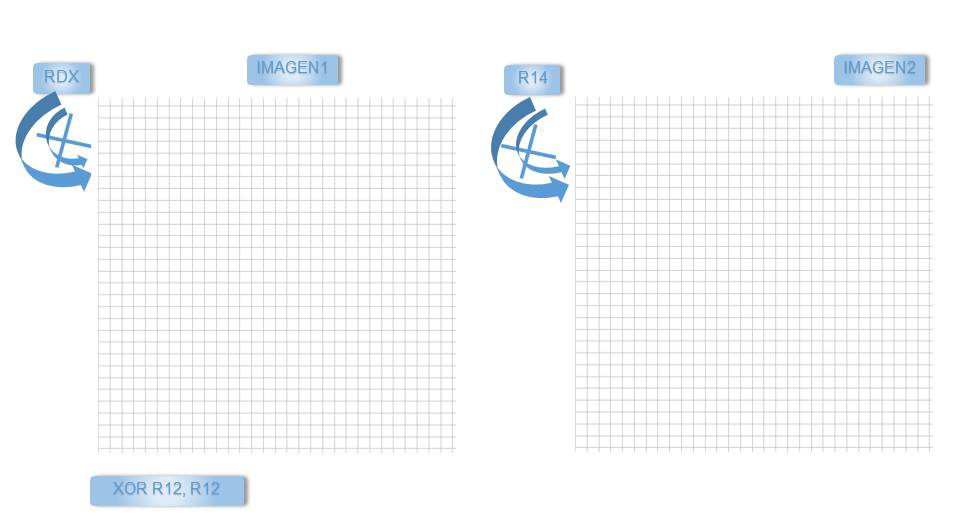
\includegraphics[width=100mm]{imagenes/merge/merge1-1.png}
\caption{Desarrollo de Merge-ASM1.}
\end{figure}

Dentro del ciclo de las columnas guardamos en dos registros xmm los cuatro píxeles de cada imagen. Luego desempaquetamos cada registro en otros dos registros para incrementar el tamaño de las componentes de los píxeles y volvemos a repetir esta operación para obtener cada pixel ocupando un registro xmm, una componente por doubleword, y así convertirlos a float.

%\begin{figure}[ht!]
%\centering
%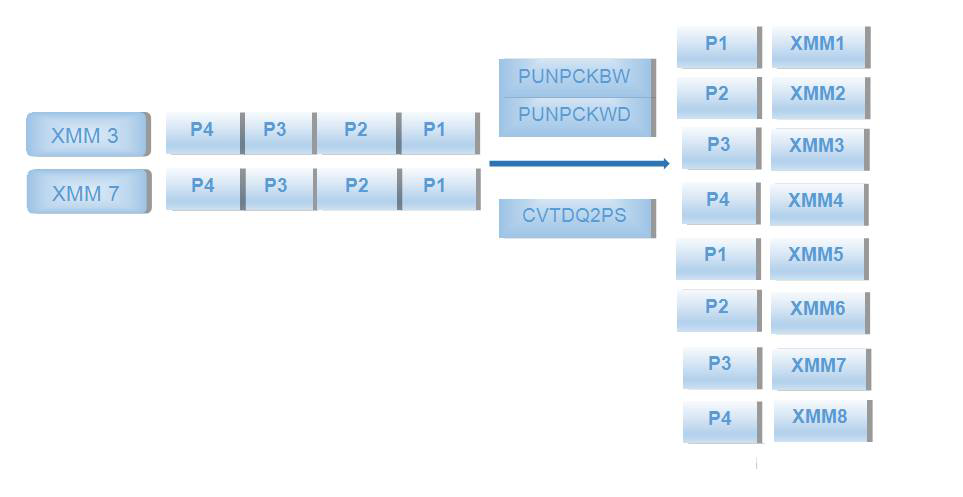
\includegraphics[width=90mm]{imagenes/merge/merge1-2.png}
%\caption{*************INSERTAR IMAGEN DE LOS XMM CORRESPONDIENTES CON LAS LOS PIXELES*************}
%\end{figure}

Luego realizamos el producto del RGB del píxel por nuestro value, dejando intacto A, y al píxel ubicado en la misma posición pero en la otra imagen hacemos el producto por 1-value. A estos valores los sumamos y convertimos a enteros, y los empaquetamos de dword a word y de word a byte para que el píxel recupere su valor original.

\begin{figure}[ht!]
\centering
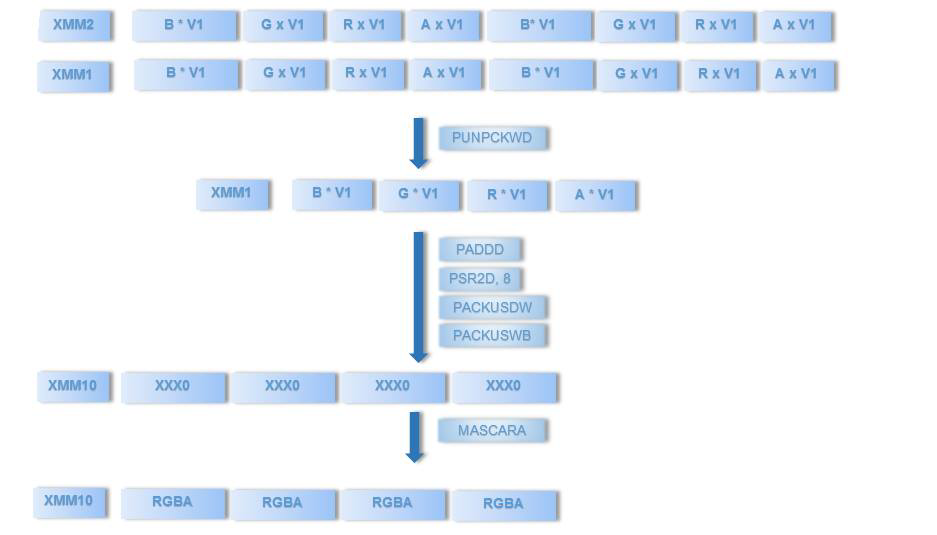
\includegraphics[width=120mm]{imagenes/merge/merge1-3.png}
\caption{Desarrollo de Merge-ASM1.}
\end{figure}

Para finalizar, volvemos a guardar el pixel en memoria y termino de realizar la iteración, para volver a comenzar a repetir el proceso con los siguientes 4 píxeles.

\subsubsection{Implementacion 2}

\textbf{Explicacion Assembler}

En la segunda implementación del filtro Merge realizamos la implementación utilizando números enteros. Como value es un float entre 0 y 1, debimos encontrar una forma de manipular la función para que use valores en entero. Por ésto, debemos multiplicar a value por 256 y guardamos su valor y su complemento en los registros XMM0 y XMM15 con tamaño word en todas las posiciones posibles de los registros. Elegimos el valor 256, ya que luego al momento de dividir, al ser una potencia de 2 nos facilita la tarea. Además, tuvimos en cuenta de no pasarnos del valor máximo posible dado la cantidad de bits de un word, al momento de realizar las operaciones, para que no se produzca overflow.

\begin{figure}[ht!]
\centering
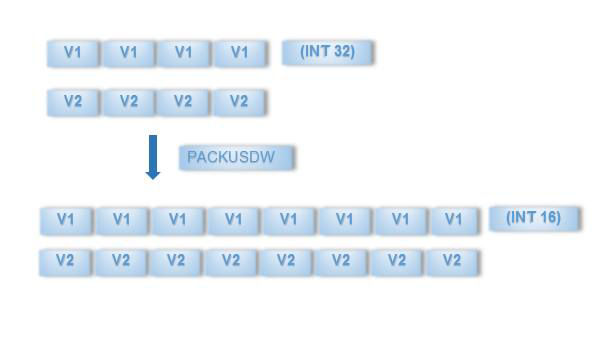
\includegraphics[width=90mm]{imagenes/merge/merge2-1.png}
\caption{Desarrollo de Merge-ASM2.}
\end{figure}

Después de realizar esta manipulación de los datos, comenzamos a operar usando 2 ciclos anidados, copiando cuatro píxeles de cada imagen los registros xmm1 y xmm5 en cada iteración. En un tercer registro, en nuestro caso xmm10, guardamos la componente A de cada pixel ya que no debe ser modificada. Luego duplicamos el tamaño de las componentes de los píxeles de xmm1 y xmm5 y guardamos 2 píxeles por registro, usando además los registros xmm3 y xmm7 para poder contenerlos a todos.

A continuación procedemos a multiplicar los píxeles de los registros por value o su complemento, dependiendo a que imagen pertenecen, expandiendo el tamaño de las componentes de los resultados obteniendo los siguientes registros:

\begin{figure}[ht!]
\centering
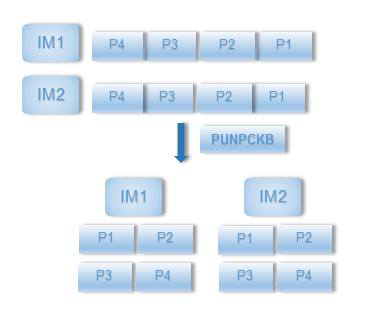
\includegraphics[width=70mm]{imagenes/merge/merge2-2.png}
\caption{Desarrollo de Merge-ASM2.}
\end{figure}

Una vez obtenidos los píxeles de esta forma, procedemos a realizar la suma de los píxeles de una imagen con los correspondientes de la otra, y dividimos cada componente por 256 (el valor utilizado al inicio para poder operar con enteros). Esta división la realizamos utilizando PSRLD XMMi, 8, que es equivalente a dividir cada componente por 256.

Finalizadas estas operaciones, continuamos por volver las componentes de los píxeles a su tamaño original, guardando los 4 píxeles en XMM1, y restaurando el valor de la componente A que habiamos guardado en XMM10.

\begin{figure}[ht!]
\centering
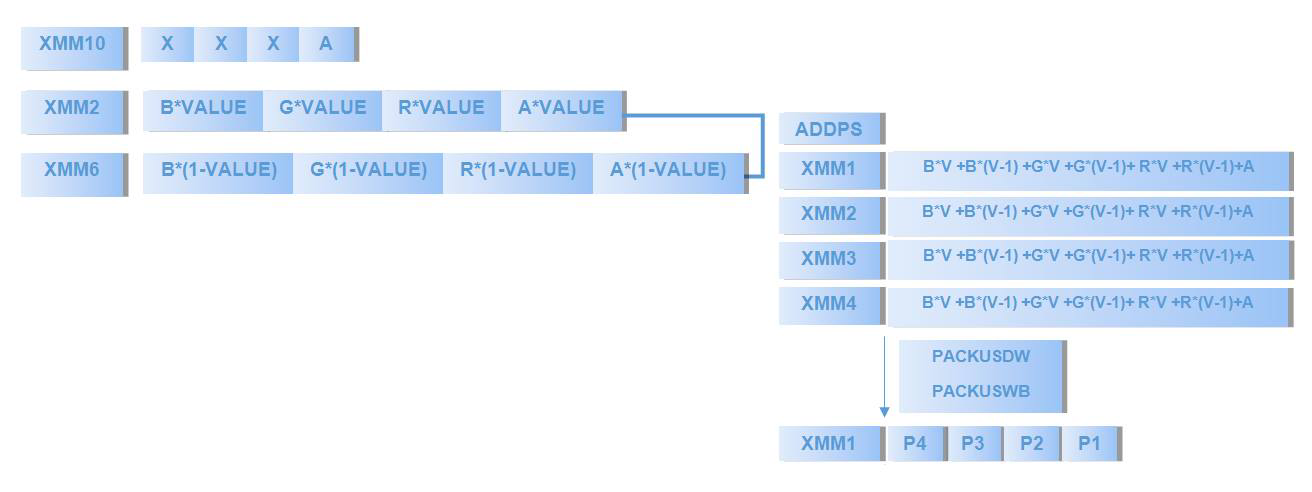
\includegraphics[width=140mm]{imagenes/merge/merge2-3.png}
\caption{Desarrollo de Merge-ASM2.}
\end{figure}

Luego de terminar con las operaciones, guardo en memoria los píxeles modificados y repito las operaciones con los siguientes 4 hasta procesarlos a todos.